%********************************************************************************************
%								COMANDOS ÚTILES PARA LATEX EN ESTE TP							
%
%	\ : espacio simple
%	\\ : nueva línea
%	\par : va a la línea de abajo y deja sangría
%	\vspace{##tamaño en pt##} o \vspace{\baselineskip} en general:
%								 para dejar un espacio vertical
%	\textbf{text} :text en negrita
%	\textit{text} :text en itálica
%
% GRAFICOS CENTRADOS:
%	\begin{center}
%		\includegraphics[width=\textwidth]{./img/##ruta imagen (no hace falta extension)##}
%	\end{center}
%		--> se pueden agregar atributos como scale por si se hace muy grande
%
% TABLAS CENTRADAS:
%	\begin{center}
%	\begin{tabular}{|c|c|}
%	\hline
%	\ \textbf{Programa} & \textbf{Ticks} \\
%	\hline
%		ASM & 675127609 \\
%	\hline
%	\end{tabular}
%	\end{center}
%
% ALGORITMOS (EN VARIOS LENGUAJES):
% \begin{lstlisting}
%	void sumoDiez(int &num)
%	{
%	    num += 10;
%	}
%	
%	int main()
%	{
% 	   int i;
%	    int numeroAProcesar = 20;
%	    for (i = 0; i < 50; i++)
%	    {
%	        sumoDiez(numeroAProcesar);	//Proceso el numero en cada ciclo
%	    } 
%	    return 0;
%	}
%	\end{lstlisting}
%
% para info sobre todo lo que tiene el package detallado:
% http://en.wikibooks.org/wiki/LaTeX/Source\_Code\_Listings
%
%********************************************************************************************

\documentclass[10pt,a4paper]{article}
\usepackage[utf8]{inputenc} % para poder usar tildes en archivos UTF-8
\usepackage[spanish]{babel} % para que comandos como \today den el resultado en castellano
\usepackage{a4wide} % márgenes un poco más anchos que lo usual
%\usepackage{geometry}

%\usepackage{layout}

%\geometry{
%  includeheadfoot,
%  margin=2.7cm
%}

\usepackage[conEntregas]{caratula}
\usepackage{amssymb}
\usepackage{fancybox}
\usepackage[usenames,dvipsnames]{color}
\usepackage{hyperref}
\usepackage{listings}
\usepackage{clrscode3e}
\usepackage{xcolor}
\usepackage{amsmath}


\hypersetup{
    colorlinks,
    citecolor=black,
    filecolor=black,
    linkcolor=black,
    urlcolor=black
}

\lstdefinestyle{customc}{
  belowcaptionskip=1\baselineskip,
  breaklines=true,
  frame=L,
  xleftmargin=\parindent,
  language=C,
  showstringspaces=false,
  basicstyle=\footnotesize\ttfamily,
  keywordstyle=\bfseries\color{green!40!black},
  commentstyle=\itshape\color{purple!40!black},
  identifierstyle=\color{blue},
  stringstyle=\color{orange},
}

\lstset{escapechar=@,style=customc}

\begin{document}

\titulo{Trabajo Práctico 2}
\subtitulo{Develando la mentira de los megapíxeles [Primera entrega]}

\fecha{\today}

\materia{Métodos Numéricos}
\grupo{Grupo Autodenominado "Los Pichis"}

\integrante{De Sousa Bispo, Germán Edgardo}{359/12}{german\_nba11@hotmail.com}
\integrante{De Sousa Bispo, Mariano Edgardo}{389/08}{marian\_sabianaa@hotmail.com}
\integrante{Valdés Castro, Tobías}{800/12}{tobias.vc@hotmail.com}


\maketitle

\tableofcontents
\newpage

\section*{Introducción}
\addcontentsline{toc}{section}{Introducción}

Luego de haber llevado a cabo el TP1 y el TP2 de métodos númericos, la excelente compañía \textbf{Adobby} se vio interesada en nosotros. En vista de que se presentaron tres puestos libres en la compañia (se dice que tres de sus empleados, un flaquito de anteojos, un colorado y una sabelotodo, partieron en búsqueda de un nuevo trabajo en ``El Que No Debe Ser Nombrado''), los recruiters de la empresa lanzaron un desafío para encontrar los reemplazantes de lo que llamaban ``el trío mágico'', y suplantarlos de esta manera en sus puestos de \textit{Ninja Gurú Jedi Master: The image demosaicing god.}

\par 
El desafío consiste en diseñar, implementar y analizar un algoritmo para resolver el
problema de demosaicing. El mismo consiste en obtener una imagen con información en los 3 canales (colores rojo, verde y azul) para cada pixel, a partir de la información capturada por un sensor de una cámara digital marca \textit{``Fotos Casi en Movimiento''}. Para esto se asume que la información captada por el sensor es
correcta y se trata de inferir los valores de los dos canales faltantes en cada uno de los píxeles de la imagen.
\par 
Con el fin de no tener que invocar artes oscuras para resolver este problema, el desafío plantea trabajar solo sobre el Bayer Array. El mismo consiste en alternar filas de rojo y verde o verde y azul. Cada color no recibe una fracción igual en el area ya que el ojo humano es mas sensitivo a la ``luz verde''. Este tipo de arreglo tiene el doble de elementos verdes que rojos o azules, lo cual produce una imagen que aparenta tener menos ruido y mayor detalle que si se trataran los tres colores por igual. El motivo por el que sucede esto escapa los efectos de este trabajo práctico.
\par 
Como parte del desafío de lo que denominaron \textit{``El torneo de los Tres Programadores''}, \textit{Adobby} pidió que se implementaran varios métodos para poder recrear la imagen a partir de lo que tomó la cámara.


\section{Desarrollo}

\subsection{Implementación}


Nuestro programa recibe como parámetros el nombre de un archivo que posee los valores de la matriz que representa la imagen obtenida por la cámara. Es decir, sin haber hecho ningun proceso de demosaicing. Además, recibe qué filtro deberá aplicarse y, en caso del algoritmo de Malvar, He y Cutler, obtiene como tercer parámetro el valor \textbf{$\alpha$}.
\par 
Lo primero que se hace es tomar el archivo obtenido por parámetro y, a partir de sus datos, crear la \textit{bayerImage} correspondiente, que luego es utilizada para aplicar el filtro correspondiente al segundo parámetro.
\par 
Finalmente, luego de la ejecución del filtro correspondiente, se guardan tres archivos correspondientes a las capas verde, azul y roja de la imagen obtenida. Estos archivos tienen un formato que permite ser leído por \textit{matlab}, desde donde posteriormente se van a recrear las imágenes.
\par 
Además, dado que en este trabajo práctico, la obtención del archivo con la representación en bayer array se hace a partir de una imagen y no de lo que capten los sensores de una cámara, el algoritmo que transforma la foto en el archivo de texto fue realizado en matlab, así como otras pequeñas cosas. Todos estos scripts se pueden encontrar en la carpeta \textit{matlab}.

\vspace{2\baselineskip}

Todas la implementaciones que se mostrarán a continuación, se hicieron bajo la base de obtener el siguiente bayer array:

	\par 
	\begin{center}
		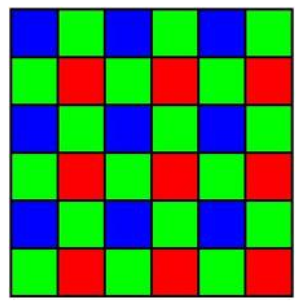
\includegraphics[scale=0.4]{./img/bayerarray.png}
		\par 
		\footnotesize\textit{Modelo de Bayer Array utilizado.}
	\end{center}
	\par 
	
Como podemos notar, e indexando las filas y columnas desde 0, los píxeles azules se encuentran en las posiciones de fila par y columna par. Por otro lado, el color rojo aparece en las filas impares y columnas impares, mientras que el color verde se encuentra en toda posición que no cumple la misma paridad entre columnas y filas.
\par 
Una vez dicho esto, comenzamos con el análisis de las implementaciones realizadas para los siguientes filtros.
	
\subsubsection{Closest Neighbor}

Este filtro se basa en rellenar los valores faltantes copiando al vecino más
cercano del pixel, siempre y cuando tenga una observación real en el mismo canal que se está tratando averiguar. Este fundamento se basa en considerar que el valor de dos pixeles cercanos no debe variar mucho respecto de un mismo canal. De esta manera, podemos obtener toda la información que necesitamos a partir de contemplar el entorno de cada pixel.
\par 
En nuestro caso, se decidió dividir los casos dependiendo si la información que buscamos corresponde al canal verde o a otro canal.
\par 
Como ya se explicó previamente, el color verde va a ser encontrado en las columnas impares y filas pares al igual que en las columnas pares y filas impares. De esta manera, y mirando el modelo de bayer array que se planteó previamente, decidimos tomar los valores que se encuentra en la fila superior y misma columna, y los valores en la columna anterior y misma fila (es decir, tomar el valor del pixel justo encima y el que se encuentra justo a la izquierda). Sin embargo, a qué canal corresponde cada valor depende de en qué fila se encuentre el pixel que quiero reconstruir. Es por esto que se hace un chequeo sobre la fila del píxel.
\par 
Solo a manera ilustrativa e informativa, se muestra en qué sector del código se realiza esto (método \textit{FilterImage()}): 
\begin{lstlisting}
if (bayerImage.CurrentPixelIsGreen(i,j))
{
	greenChannelValue = bayerImage.GetPixel(i, j);
	blueChannelValue = getBlueChannelInGreenPixel(i, j);
	redChannelValue = getRedChannelInGreenPixel(i, j);
}
\end{lstlisting}
\par 
Donde \textit{getBlueChannelInGreenPixel(i,j)} y \textit{getRedChannelInGreenPixel(i,j)} hacen la deferencia sobre en que fila se encuentra el pixel con valor de verde para devolver correspondientemente el color azul y rojo.
\par
A continuación de esto se plantea el caso en el que \textbf{NO} estamos ubicados en un pixel verde. Nuevamente, mirando el modelo utilizado para el bayer array, suceden dos casos: o el pixel es azul o es rojo. Sin embargo, en ambos se puede encontrar un pixel verde a su lado izquierdo (hay que ver cuestiones de bordes que serán explicadas a continuación). Y a su vez, en cualquier diagonal contigua podemos encontrar el otro color distinto de verde, es decir, al azul si estamos en rojo y viceversa. Elegimos tomar el valor que se encuentra en la diagonal superior izquierda. El código para esta parte es muy similar al mostrado previamente, solo que las condiciones son distintas. Igualmente, la asignación a las variables se hace de la misma forma.
\par 
Debido a lo recién mencionado, se hace una distinción en todo momento acerca de qué color es el pixel que estamos utilizando. De esta manera podemos elegir cuál posición vecino corresponde al mismo canal que mi pixel para tomar su valor. Cabe destacar que la elección de estos vecinos fue arbitraria. Dependiendo de la imagen que se utilice, algún vecino puede funcionar mejor que otra, pero esto no es cuantificable ni sigue un patrón tal que elegir un vecino en particular sea siempre la mejor opción.
\par 
Debido a que siempre estamos completando la información faltante a partir de los píxeles que se encuentran en la fila superior o la columna anterior (mirando de izquierda a derecha), el filtro comienza a aplicarse a partir de la segunda fila y la segunda columna. De esta manera, el primer caso será a partir de la posición $(1,1)$ de la matriz (indexada desde 0). Luego, en \textit{matlab} se le recorta el borde a la imagen, dejando sin utilización así el borde para el cual se perdió la información.
\par 
Finalmente, se setean los valores obtenidos a los canales correspondientes.



\subsubsection{Bilinear Interpolation}
Este es un método que se compone de sucesivas interpolaciones lineales. De esta manera, se aproxima el valor de una función de dos variables a partir de puntos cercanos al que se quiere averiguar. En nuestro caso, esto se trasmite a cada pixel.  
\par 
Primero empecemos diciendo que es la interpolación lineal:
La interpolación lineal fue definida como \textit{$(aValue + anotherValue)/2.0$}, siendo $aValue$ y $anotherValue$ los valores de los pixeles que se desean interpolar. 
\par 
De esta manera, nuestra interpolación bilineal consiste en hacer dos interpolaciones lineales, por ejemplo, una en las filas y otra en la columna, y luego interpolar linealmente ambos resultados.
\par 
Este caso sucede explicitamente cuando se desea interpolar para obtener los valores rojo y azul de un pixel verde. Haciendo referencia al ejemplo de Bayer Array, cuando nos encontramos con un pixel verde, podemos tener a ambos lados píxeles rojos o azules. Dependiendo de cual de estos casos cumplamos, arriba y abajo vamos a tener el color opuesto. De esta forma, cuando estemos en un pixel verde, se obtendrá el color azul interpolando linealmente verticalmente u horizontalmente (dependiendo de si estamos en fila par o impar), lo cual se repetirá en el sentido opuesto para el rojo, obteniendo así los valores correspondientes a azul y rojo.
\par 
La recreación del color verde se genera a partir de los píxeles azules y rojos. Como se puede ver en el bayer array, cuando estamos en un pixel azul o rojo, tanto encima o abajo y a derecha e izquierda tenemos píxeles verdes. De esta manera, tomamos los cuatro píxeles verdes aledaños para realizar la interpolación; por un lado horizontalmente y luego verticalmente, para finalizar interpolando ambos resultados. 
\par 
En estos casos, también debemos obtener el color distinto de verde contrario al cual ya tenemos. Para estos casos, desplazándose en cualquier diagonal podemos encontrar píxeles de ese color. Por lo que en nuestra implementación se hace una interpolación lineal para ambos pixeles en la fila anterior y otra para los de la siguiente fila. Finalmente, se interpolan entre ellos obteniendo el valor objetivo.
\par 
La decisión de tomar los píxeles mencionados para realizar las interpolaciones, al igual que en \textit{Closest Neighbor}, fue arbitraria. El factor más influyente fue la cercanía entre píxeles, ya que como se mencionó en la sección previa, se espera que los valores no varíen demasiado de un píxel a otro. De esta manera, e interpolando los puntos cercanos, se espera obtener un valor mucho más cercano que simplemente tomar alguno de los vecinos y utilizarlo.
\par 
%VER SIGUIENTE FRASE
Debido a la forma en la que fue realizada el código, y gracias al polimorfismo, el código que resuelve el filtro de imagen es igual al utilizado en \textit{Closest Neighbor}. La única variación corresponde al código que devuelve los valores de los colores obtenidos. Para el caso de interpolación bilineal, se realizó lo explicado previamente.

\subsubsection{Directional Interpolation}

Este método se basa en la interpolación por direcciones. En nuestro caso, esto implica interpolar valores obtenidos a partir de una dirección en la matriz. 
\par 
En nuestro caso, utilizamos el gradiente para decidir si nos convenía tomar una dirección horizontal o vertical. Mientras mayor sea el gradiente, mayor es la variación de color entre un pixel y otro. De esta manera, tomamos la dirección que menor gradiente aportaba. 
\par 
A través de splines (con el algoritmo obtenido del libro \textit{``Numerical Analysis'' de Richard L. Burden y J. Douglas Faires}, obtuvimos todos los polinomios correspondientes a la fila o la columna correspondiente al pixel del que deseamos obtener la información faltante. De esta forma, interpolamos, particularmente, el punto (en nuestro caso, pixel) del cual queremos obtener la información.



\subsubsection{Algoritmo de Malvar, He y Cutler}


\subsubsection{Problemas en la Implementación}

	
\subsection{Experimentación}


\subsubsection{Análisis Cuantitavo}

\subsubsection{Análisis Cualitativo}

Comparando directional y malvar-he-cutler: el directional blurea los bordes. A veces mejora pero si no hay un cambio brusco en los colores (como en el pico), se blurea mucho. Y malvar con 1/2 alfa queda bien, pero queda con zipping en los bordes negros.


\section{Conclusión}


\section{Bibliografía y referencias} %arreglar cuando se termine 

\begin{itemize}
	\item \textbf{STL de C++}: \url{http://en.cppreference.com}.
%	\par Para la función \texttt{rand()}, \url{http://en.cppreference.com/w/cpp/numeric/random/rand}.
%	\par Para la función \texttt{sort()}, \url{http://en.cppreference.com/w/cpp/algorithm/sort}.
%	\item Distribución de \texttt{rand()}?, \url{http://eternallyconfuzzled.com/arts/jsw\_art\_r and.aspx}
%	\item \textbf{Métodos Numéricos:}
%		\par Método de la potencia: Richard BURDEN, Numerical Analysis 9th Ed. Chapter 9 Section 3, p. 576
%		\par \textit{Papers} del TP.
%	\item \textbf{Contador de clocks}: \url{http://www.mcs.anl.gov/\~kazutomo/rdtsc.html}
http://www.cambridgeincolour.com/tutorials/camera-sensors.htm
http://ins.sjtu.edu.cn/people/mtang/textbook.pdf
\end{itemize}


\end{document}
